\documentclass[11pt,a4paper]{article}
\usepackage[margin=22mm]{geometry}
\usepackage{xeCJK,amsmath,amssymb,tikz}
\IfFontExistsTF{Songti SC}{\setCJKmainfont{Songti SC}}{\setCJKmainfont{FandolSong-Regular.otf}}
\usetikzlibrary{arrows.meta,calc,angles,quotes}
\pagestyle{empty}
\setlength{\parindent}{2em}
\setlength{\parskip}{5pt}
\begin{document}
\begin{center}\Large 光滑斜面上的滑块\end{center}
一个小物块从静止开始沿固定的光滑斜面下滑。斜面倾角为 $30^\circ$，物块沿斜面滑行 $2.0\,\mathrm m$，取 $g=10\,\mathrm{m\,s^{-2}}$。求此时物块的速度大小。
\begin{center}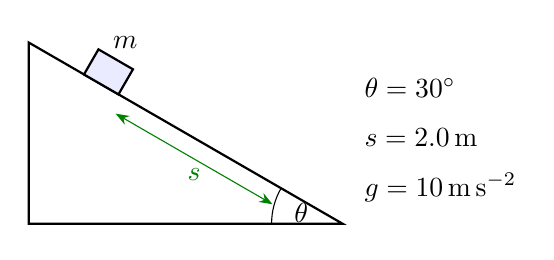
\begin{tikzpicture}[>=Stealth,scale=1.15]
\coordinate (A) at (0,2);\coordinate (B) at (3.464,0);\coordinate (C) at (0,0);
\draw[thick] (A)--(B)--(C)--cycle;
\draw pic[draw,angle radius=9mm,"$\theta$"] {angle=A--B--C};
\begin{scope}[shift={(0.8,1.538)},rotate=-30]
\draw[fill=blue!8,thick] (-.22,0) rectangle (.22,.32);
\node at (0,.53) {$m$};
\draw[<->,green!50!black] (.3,-.2)--(2.3,-.2) node[midway,below] {$s$};
\end{scope}
\node[right] at (3.6,1.5) {$\theta=30^\circ$};
\node[right] at (3.6,.95) {$s=2.0\,\mathrm m$};
\node[right] at (3.6,.4) {$g=10\,\mathrm{m\,s^{-2}}$};
\end{tikzpicture}
\end{center}

已知斜面固定、接触面光滑，物块可视为质点。请画出受力图，沿斜面列运动方程，再求末速度。
\end{document}
